\chapter{The Study of H$\alpha$ Emission Spectra}

\section{Context and Relevance}
P Cygni and inverse P Cygni spectra are sub classes of H$\alpha$ emission spectra \cite{zhang2021catalog}. The identification of H$\alpha$ emission spectra in large scale spectroscopic surveys is an active area of research.\cite{zhang2021catalog,vcotar2021galah,traven2015gaia}. Thus the identification of H$\alpha$ emission spectra can serve as a useful precursor to identifying P Cygni and inverse P Cygni spectra. This approach can be extremely beneficial in reducing the search space as well the feature space that may serve as input data to a detection and identification pipeline that is tuned to identify P Cygni and inverse P Cygni spectra. 

This chapter presents a brief summary of recent methods employed to identify H$\alpha$ emission spectra, in both smaller scale observations as well as large scale surveys. These are placed in the context of their importance in the identification of P Cygni and inverse P Cygni spectra.

\section{A Historical Perspective}
An atlas of high resolution line profiles with H$\alpha$ emissions was provided by Vam Winckel at al. in 1993\cite{van1993atlas}. The authors provide a classification scheme for H$\alpha$ spectra based on their morphology. The spectra were identified and classified using manual methods. Direct visual inspection and measurement of the width and shape of the line profile was used to classify these spectra. In particular, wind velocity dispersions outside the primary disk of the star were used to determine the membership of candidates in each class.
A few of the classes identified by the authors include, subtype S1, narrow emission with no prominent absorption; subtype S2 which shows a clear absorption feature superimposed on a broad emission feature; and subtype S3 which shows a strong absorption feature which reaches at least the continuum level. The authors note that the radial velocities of the 59 emission lines considered were generally redshifted. It is noteworthy that this study used wind velocity dispersions to classify the spectral types. For example, S3 showed the smallest wind velocity dispersion, thus demonstrating a relationship between the morphology of the spectra and the physical processes that generate them.

\begin{figure}[h]
\centering
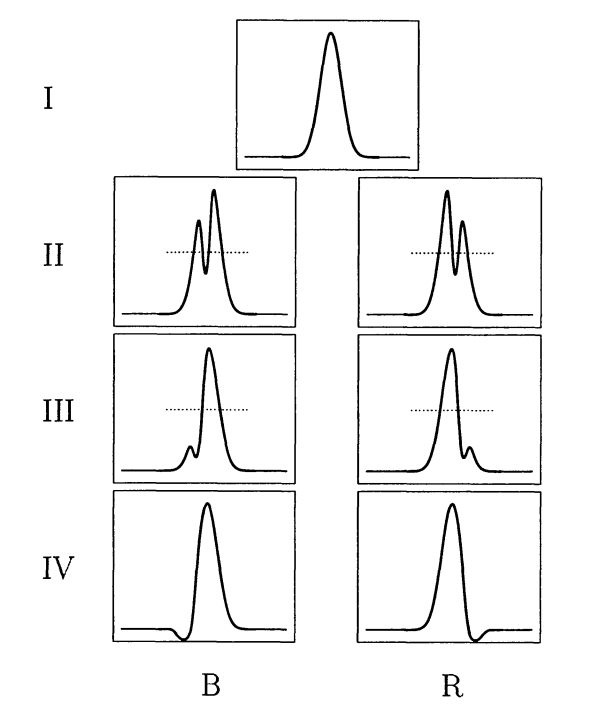
\includegraphics[scale=0.75]{figures/reipurth classes.png}
\caption{The morphology based classification scheme proposed by Reipurth et al. Depending on the location of the primary peak in relation to the secondary peak, the letters B and R are appended to the Roman numerals. They stand for blue-shifted and red-shifted respectively.}
\end{figure}

Published in 1996, Reipurth et al. studied the H$\alpha$ profiles of pre-main sequence stars using manual methods. In addition to identifying T Tauri stars and Ae/Be stars using high resolution spectra (R~50,000), the study focused on the morphological properties of P Cygni stars as well as the physical processes that generate them. The study notes the discovery of complex morphological profiles among the T Tauri, Ae/Be and P Cygni stars. 

The authors proposed a two dimensional classification scheme based on the relative height of a secondary peak compared to the primary peak, as well as whether the absorption line is blue or red shifted. The authors note the classification of 25\% symmetric profiles, 49\% blue shifted absorption profiles and 5\% P-Cygni profiles amongst the observed spectra. Of the spectra, 21\% fall into the redshifted absorption category. In addition to this morphological classification, the authors also presented wind velocities of the samples with some stars recording extremely high velocities of ~ 900km/s \cite{reipurth1996halpha}. 

The classification of P Cygni stars in this paper follow the scheme proposed by Beals in 1953\cite{1953PDAO....9....1B}. The authors have also presented a discussion comparing observed data to models in literature, particularly models that constrain mass, radii and photospheric temperatures. No specific model details for P Cygni stars were provided. Further catalogues of H$\alpha$ emission stars have been provided by Kohoutek and Wehmeyer (1997 and 1999). These catalogues contain 98 identified emission-line stars in the Northern Milky Way. These catalogues do not specifically identify P Cygni stars or inverse P Cygni stars \cite{kohoutek1999catalogue}.

The study of open clusters such as NGC 6611 and others have pushed our understanding of H$\alpha$ emission stars \cite{bonito2013spectroscopic,traven2015gaia}. Bonito et al. in particular note that for stars surrounded by active disks the morphology of the emission lines could fall into categories such as symmetric with broad wings, asymmetric and in extreme cases, P Cygni and inverse P Cygni. The authors have used the classification scheme proposed by Reipurth et al and have adhered to the type I - IV scheme with B and R suffixes to denote blu shifted and red shifted emission lines respectively. The historical review allow us to draw a number of conclusions:

\begin{enumerate}
\item These methods relied exclusively on visual inspection of spectra and manual methods to identify H$\alpha$ candidates. While this may have been a suitable approach in the past, it is extremely challenging to extend and scale these methods to datasets generated by million star all sky surveys in the modern era. Thus this project does not consider these manual methods for the detection of H$\alpha$ candidates as well as P Cygni and inverse P Cygni spectra. 

\item Morphology based classification approaches as demonstrated by Reipurth et al. and even Beals are significantly important. It was demonstrated in Chapter 1 that the variety of spectral morphologies are hypothesised to be generated due to distinct physical phenomena linked to the stellar disk and the gas that surrounds it. This research leans into this approach and relies on morphological similarities and dissimilarities as a basis for spectral classification.

\item Finally, these studies have identified P Cygni and inverse P Cygni (among other classes of spectra) as forming a subset of H$\alpha$ emission spectra. This project exploits this fact to it's logical conclusion i.e. the probability of automated detection of P Cygni and inverse P Cygni spectra can be increased if the search space and feature space of the raw data can be reduced from the complete DR3 catalog, to a much narrower subset of H$\alpha$ emission candidates identified in DR3.
\end{enumerate}

\section{Recent Developments}

The increase in data availability via large scale spectroscopic surveys has necessitated and demanded the use of semi automated and fully automated methods. Morphology based classification has been adopted by many researchers in the field and augmented by statistical methods and machine learning. In general, machine learning approaches can fall into two categories; supervised and unsupervised learning. The former relies on the availability of a suitably robust set of training examples while the latter attempts to generalise and learn from unlabelled data \cite{hastie2009elements}. A full discussion and review of machine learning methods is beyond the scope of this thesis. Techniques and methods that are relevant to this research are presented in text. Chapter 4 in particular will present a more detailed discussion on methods that are relevant to the present thesis. This section reviews four recent approaches that rely on machine learning to detect and characterise H$\alpha$ candidates, their strengths and limitations. 



